%------------------------------------------------
%	PACKAGES AND THEMES
%------------------------------------------------

% this is a 4:3 layout.
\documentclass{beamer}
% for 16:9 use this command:
% \documentclass[aspectratio=169]{beamer}

\mode<presentation> {
\usetheme{metropolis}
\setbeamertemplate{caption}[numbered]
\setbeamertemplate{navigation symbols}{} % hide navigation symbols
}

\usepackage{graphicx} % images
\usepackage{algorithm2e}
\usepackage{mathtools}
\DeclarePairedDelimiter{\ceil}{\lceil}{\rceil}
\usepackage{algpseudocode}
\usepackage{booktabs} % allows the use of \toprule, \midrule and \bottomrule in tables
\usepackage[ngerman]{babel}
\usepackage[utf8]{inputenc}
\usepackage[T1]{fontenc}
\usepackage{mathtools}
\usepackage{xcolor}
\usepackage{listings} % code
\usepackage{pgf,tikz} % drawing
\usepackage{pifont} % new symbols
\usepackage{hyperref} % pretty links
% \usepackage{algorithmicx}
% \usepackage{algpseudocode}
% \usepackage[linesnumbered,ruled]{algorithm2e}

\usepackage{lmodern}
\usepackage{subcaption}
\usepackage{textcomp}
% \usepackage{array}
% \usepackage{longtable}
% \usepackage{verbatim}
%\usepackage{tabularx}
\captionsetup[figure]{font=footnotesize}

\usepackage{amsmath}
\usepackage{amssymb}
\usepackage{amsthm}
% \usepackage{comment}
% \usepackage{enumitem}
% \usepackage[binary-units=true]{siunitx}
% \usepackage{thmtools}
\usepackage{csquotes}
\usepackage{tikz}
\usepackage{float}
\usetikzlibrary{automata,positioning}

% color settings for links
\hypersetup{
    colorlinks=true,
    urlcolor=blue,
    linkcolor=black,
    citecolor=green!50!black
}

\definecolor{mygreen}{RGB}{1,135,1}

\newcommand{\cmark}{\ding{51}}  % checkmark
\newcommand{\xmark}{\ding{55}}  % xmark
\newcommand\scalemath[2]{\scalebox{#1}{\mbox{\ensuremath{\displaystyle #2}}}}

\setbeamerfont{bibliography item}{size=\footnotesize}
\setbeamerfont{bibliography entry author}{size=\footnotesize}
\setbeamerfont{bibliography entry title}{size=\footnotesize}
\setbeamerfont{bibliography entry location}{size=\footnotesize}
\setbeamerfont{bibliography entry note}{size=\footnotesize}

% \useoutertheme{miniframes} % navigation design
\useinnertheme{circles} % use non shiny circles (itemize, etc.)

% Main slide colors
% dunkel, hell, mittel
% \definecolor{pale}{RGB}{232, 236, 237}
% \definecolor{prim}{RGB}{53, 109, 120}
% \definecolor{sec}{RGB}{104, 170, 183}
% \definecolor{tert}{RGB}{109, 155, 168}
% \definecolor{quat}{RGB}{9, 59, 68}

\definecolor{pale}{RGB}{255, 255, 255}
% \definecolor{prim}{RGB}{153, 194, 173}
% good: \definecolor{prim}{RGB}{27, 33, 42}
\definecolor{prim}{RGB}{32, 43, 50}
\definecolor{sec}{RGB}{217, 232, 224}
\definecolor{tert}{RGB}{0, 82, 41}
% save
\definecolor{quat}{RGB}{0, 82, 41}

\setbeamercolor{palette primary}{bg=prim,fg=pale}
\setbeamercolor{palette secondary}{bg=sec,fg=pale}
\setbeamercolor{palette tertiary}{bg=tert,fg=pale}
\setbeamercolor{palette quaternary}{bg=quat,fg=pale}
\setbeamercolor{structure}{fg=prim} % itemize, enumerate, etc
\setbeamercolor{section in toc}{fg=prim} % TOC sections

% Block colors
\definecolor{example_color}{RGB}{93, 137, 98}
\definecolor{alert_color}{RGB}{175, 79, 72}

\setbeamercolor{normal text}{fg=prim!20!black,bg=pale!25!white}
\setbeamercolor{alerted text}{fg=alert_color!25!black}
\setbeamercolor{example text}{fg=example_color!25!black}

\setbeamercolor{block title example}{fg=white,bg=example_color}
\setbeamercolor{block body example}{fg=black,bg=example_color!10!white}
\setbeamercolor{block title alerted}{fg=white,bg=alert_color}
\setbeamercolor{block body alerted}{fg=black,bg=alert_color!10!white}

% Override palette coloring
\setbeamercolor{subsection in head/foot}{bg=quat,fg=pale}

\setbeamertemplate{frametitle}{%
    \nointerlineskip%

    \begin{beamercolorbox}[wd=\paperwidth,ht=2.5ex,dp=1ex]{frametitle}
        \hspace*{1ex}\insertframetitle%
        \ifx\insertframesubtitle@empty\else%
        {~\tiny\textcolor{quat!35!black}{\insertframesubtitle}}%
        \fi%
    \end{beamercolorbox}%
}

% math-command for bigger norm
\newcommand\norm[1]{\left\lVert#1\right\rVert}

% use this to include other files
% in this case style definitions for code
% alternative: \include{dateiname}
\lstdefinestyle{latex}{
    language=[LaTeX]TeX,
    inputencoding=utf8,
    basicstyle=\ttfamily,
    keywordstyle=\color{blue!60!black}, % use 60 percent blue and 40 black
    commentstyle=\color{cyan!60!black},
    tabsize=2,
    emph={document,itemize,enumerate,center,tabular,table,
    figure,wrapfigure,minipage,columns,align,bmatrix,
    lstlisting,beamer,frame,tikzpicture},
    emphstyle=\color{magenta!60!black},
    morekeywords={lstset,includegraphics,theenumi,labelitemi,column,color,url,href}
}

\lstdefinestyle{inline_latex}{
    language=[LaTeX]TeX,
    inputencoding=utf8,
    basicstyle=\ttfamily,
    resetmargins= true,
    belowcaptionskip=0pt,
    aboveskip=0pt,
    belowskip=0pt,
    keywordstyle=\color{blue!60!black},
    commentstyle=\color{cyan!60!black},
    emph={document,itemize,enumerate,center,tabular,table,
    figure,wrapfigure,minipage,columns,align,bmatrix,
    lstlisting,beamer,frame,tikzpicture,Parameter},
    emphstyle=\color{magenta!60!black},
    morekeywords={lstset,includegraphics,theenumi,labelitemi,column,color,url,href,Befehlsname}
}

\lstdefinestyle{cpp}{
    language=C++,
    basicstyle=\ttfamily,
    keywordstyle=\color{blue!90!black},
    stringstyle=\color{magenta!60!black},
    commentstyle=\color{green!35!black},
    morecomment=[l][\color{gray!60!black}]{\#},
    tabsize=2
}

\lstdefinestyle{empty}{
    basicstyle=\rmfamily,
    keywordstyle=\bfseries,
    commentstyle=\color{black}\itshape
}

\lstset{style=latex}

%------------------------------------------------
%	TITLE PAGE
%------------------------------------------------

\selectlanguage{ngerman}
\title[]{Execution Monitoring for Long-Term Autonomous Plant Observation with a Mobile Robot}

\author{Tim Bohne}
\institute[]
{
\textit{AG Knowledge-Based Systems}\newline
\textit{DFKI Plan-Based Robot Control Group}
\medskip
}
\date{\today}

% make slide at the beginnig of each section
\AtBeginSection[]{
{\setbeamercolor{background canvas}{bg=white}}}

% where images are locatied
\graphicspath{{./images/}}

\begin{document}

\begin{frame}[plain] % plain slides dont have navigation bars etc.
\titlepage % Print the title page as the first slide
\end{frame}

\begin{frame}
\frametitle{Übersicht} % table of contents slide
\tableofcontents
\end{frame}

% %------------------------------------------------
% \section{Motivation}
% %------------------------------------------------

\begin{frame}
  \frametitle{Langzeit-Autonome Mobile Roboter}
  \textbf{Langzeit}\newline
  \begin{figure}[H]
    \centering
    \begin{subfigure}[b]{0.32\textwidth}
      \centering
      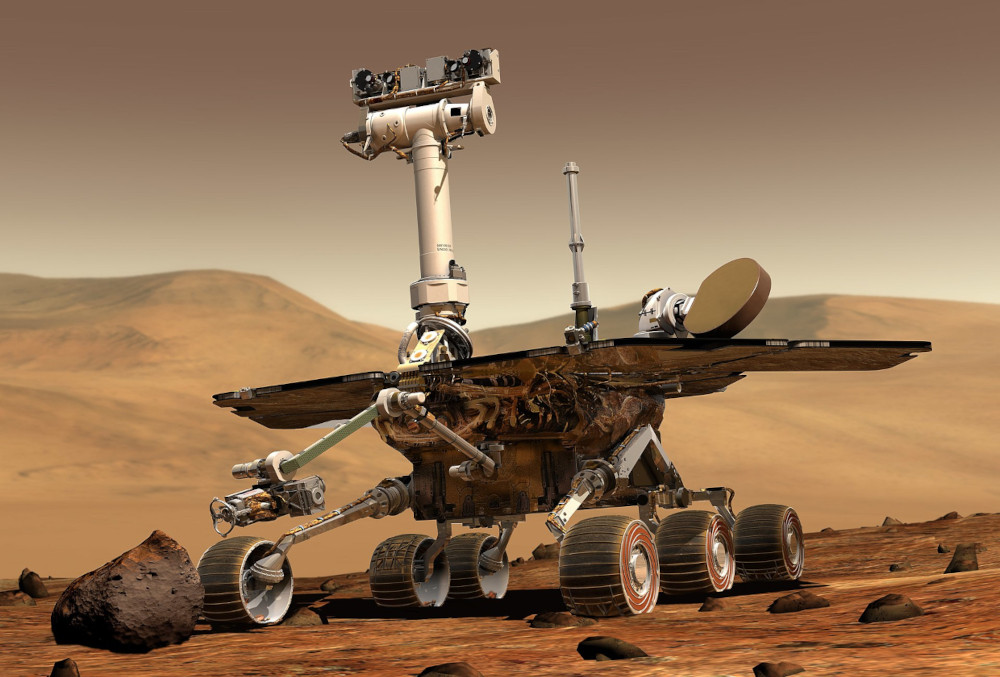
\includegraphics[width=\textwidth]{img/mars_rover.jpg}
      \caption*{$\approx$ Jahre \cite{PixelMatrix}}
    \end{subfigure}
    \begin{subfigure}[b]{0.32\textwidth}
      \centering
      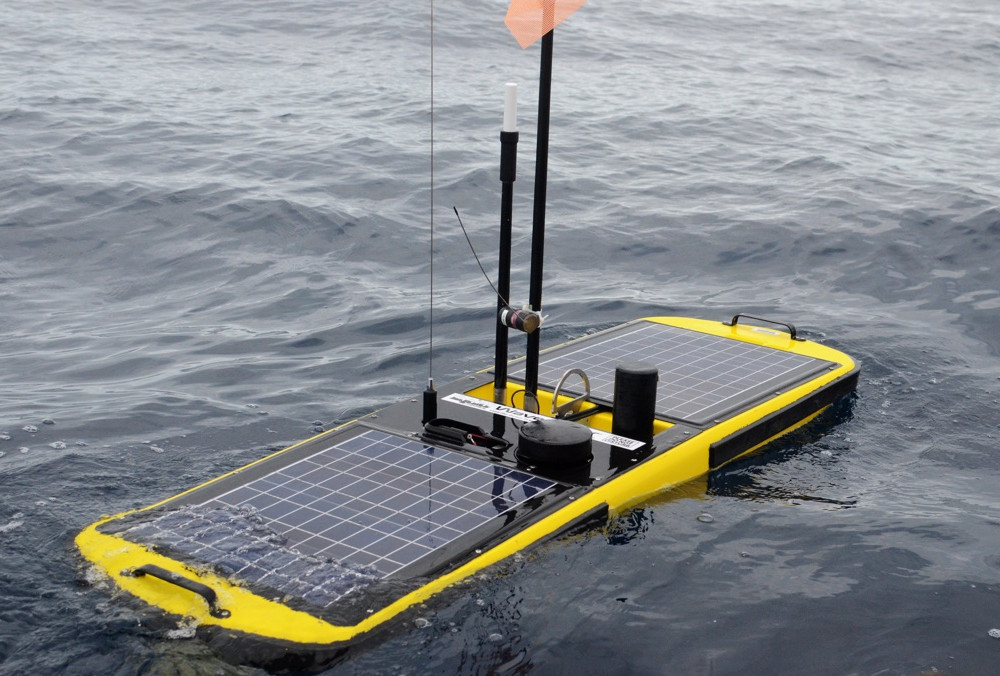
\includegraphics[width=\textwidth]{img/waveglider.jpg}
      \caption*{$\approx$ Monate \cite{Convolution}}
    \end{subfigure}
    \begin{subfigure}[b]{0.32\textwidth}
      \centering
      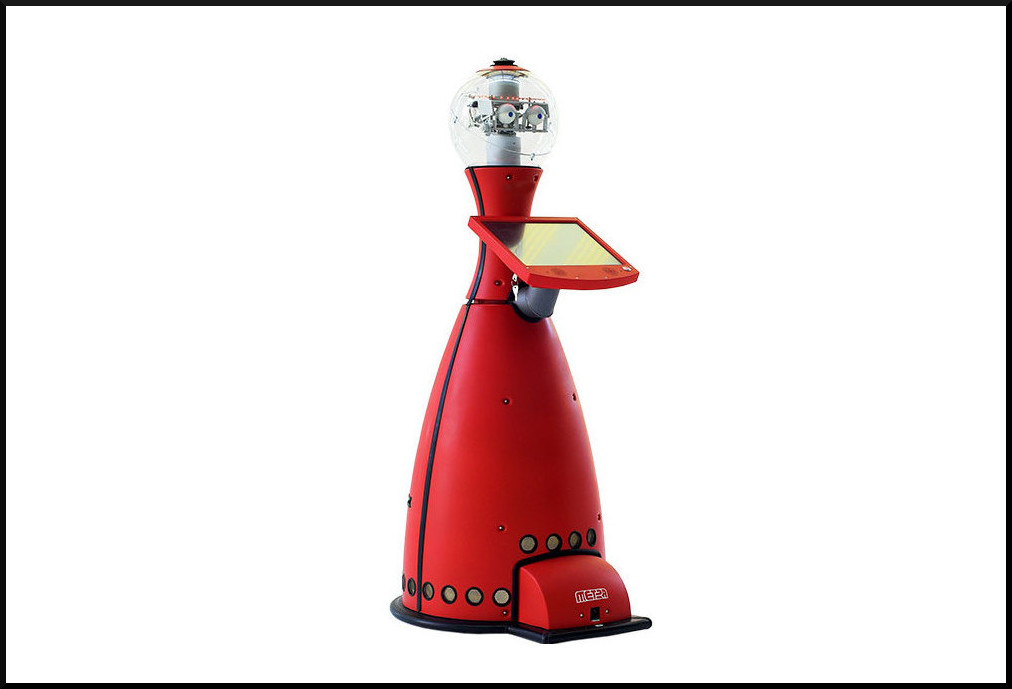
\includegraphics[width=\textwidth]{img/service_robot.jpg}
      \caption*{$\approx$ Wochen \cite{Convolution}}
    \end{subfigure}
  \end{figure}
  \begin{itemize}
    \item Keine strikte Definition \textrightarrow \thinspace \textbf{kontextabhängig}
    \item Hier: \textbf{Zeitlicher Handlungsradius des Roboters}
    \begin{itemize}
      \item Ladezyklus
      \item Missionszyklus
    \end{itemize}
    \item \textbf{LB}: Prozesse, die eine Reihe solcher Zyklen erfordern
    \item \textbf{UB}: Wartungsintervalle
  \end{itemize}
\end{frame}

\begin{frame}
  \frametitle{Langzeit-Autonome Mobile Roboter}
  \textbf{Autonomie}
  \begin{itemize}
    \item Ebenfalls nicht scharf definiert und \textbf{kontextabhängig}
    \item \textbf{Kooperation} nicht prinzipiell ausgeschlossen
    \item Hier: \textbf{Vollautonom} - Inanspruchnahme menschlicher Hilfe ausschließlich im Fehlerfall
  \end{itemize}
  \begin{figure}[H]
    \centering
    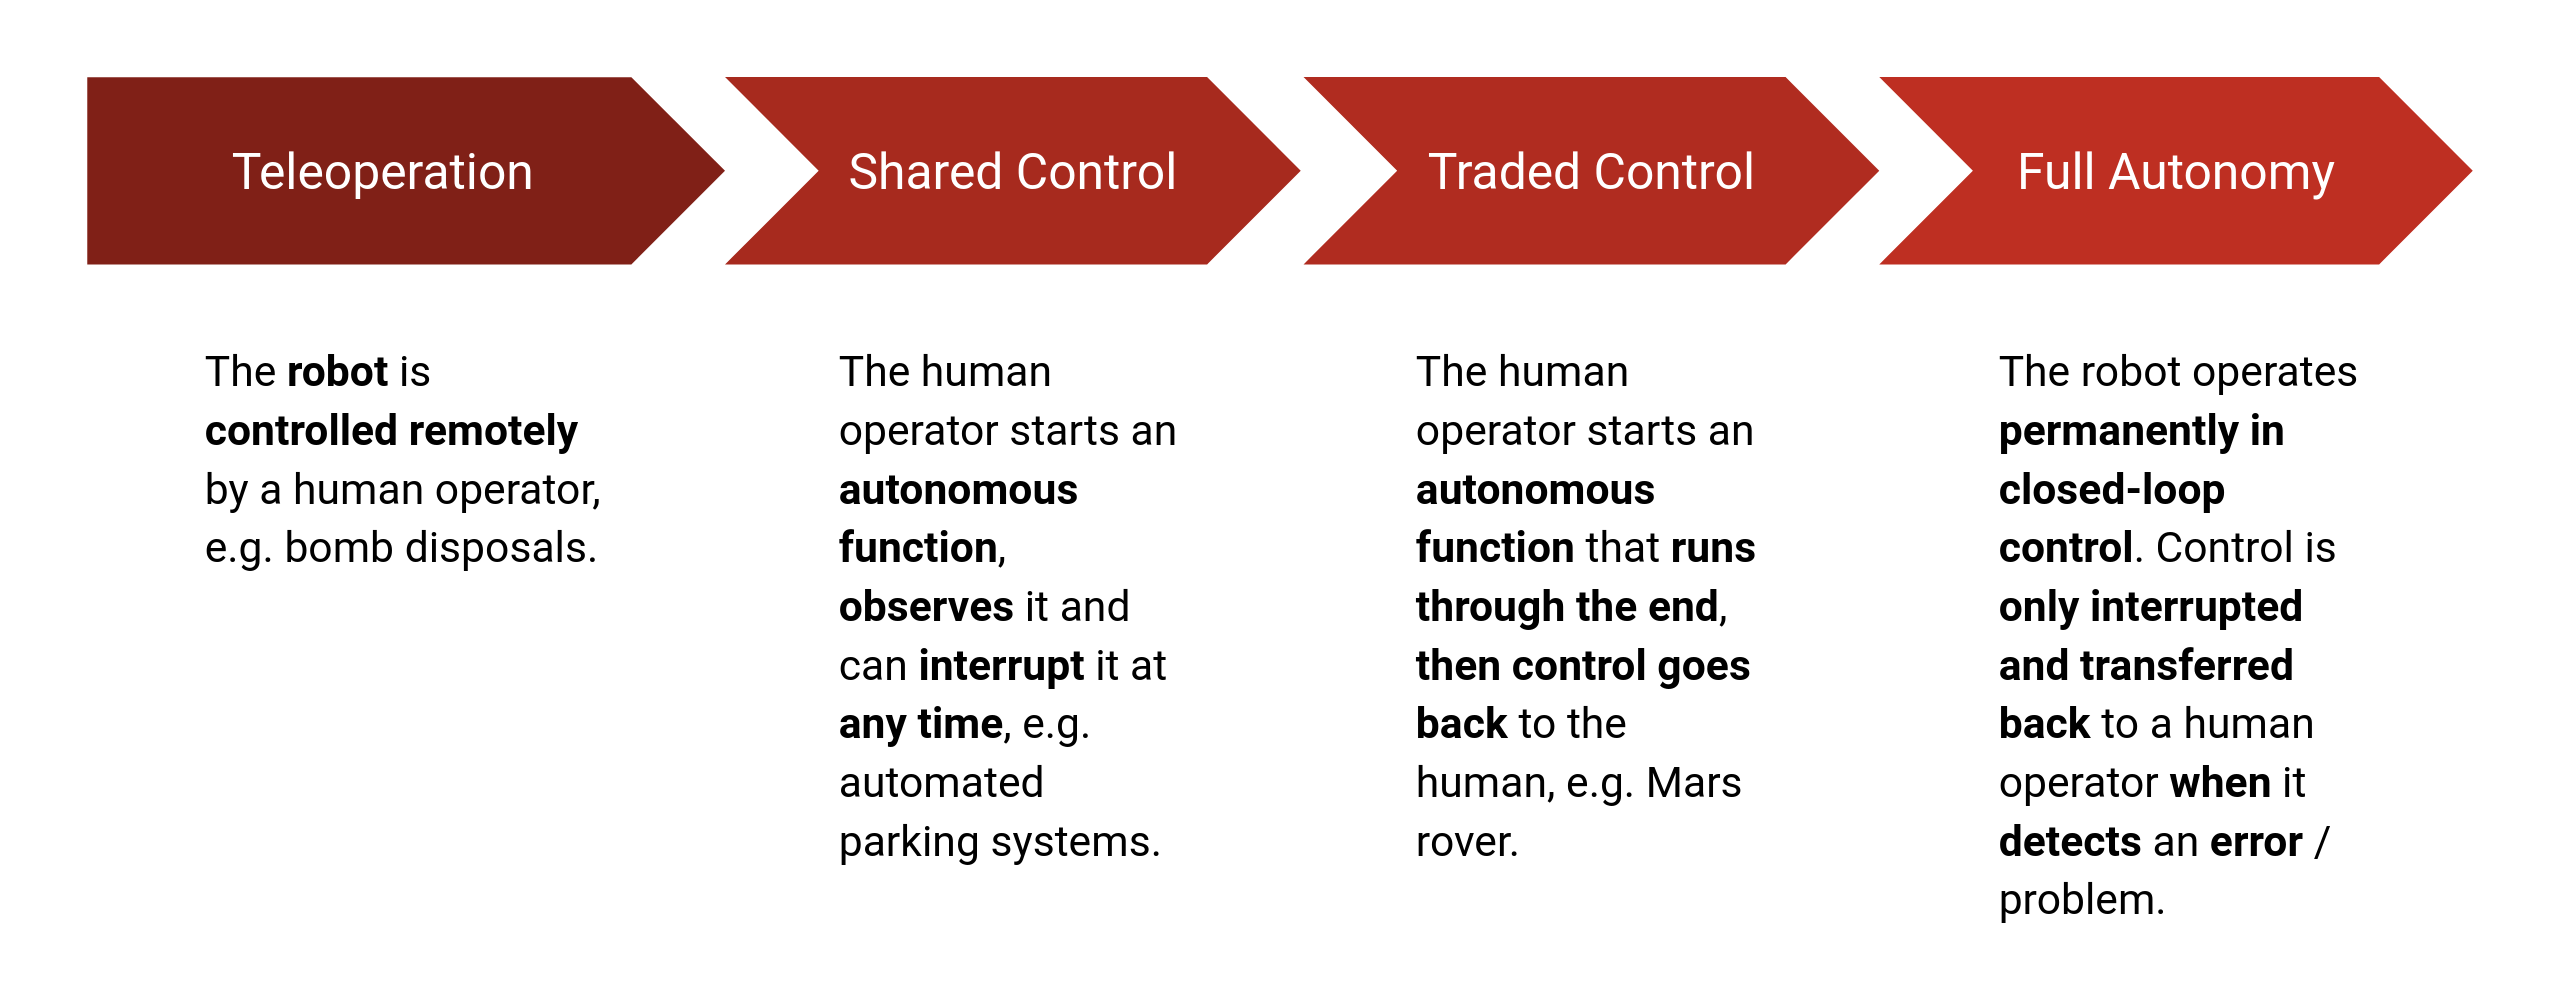
\includegraphics[width=\textwidth]{img/autonomy_spectrum.png}
    \caption*{Spektrum der Autonomie}
  \end{figure}
\end{frame}

\begin{frame}
  \frametitle{Langzeit-Autonome Mobile Roboter}
  \textbf{Mobil}\newline
  System, das in der Lage ist, sich innerhalb bestimmter Grenzen frei in einer Umgebung zu bewegen.
\end{frame}

% % %------------------------------------------------
% % \section{Graph Neural Networks (GNNs)}
% % %------------------------------------------------

% %------------------------------------------------
% \section{Robustheit}
% %------------------------------------------------

% %------------------------------------------------
% \subsection{GNNs: Manipulation der Knoten-Attribute}
% %------------------------------------------------

% %------------------------------------------------
% \subsection{GNNs: Manipulation der Graph-Struktur}
% %------------------------------------------------

% %------------------------------------------------
% \section{Fazit / Ausblick}
% %------------------------------------------------

\begin{frame}[allowframebreaks]
  \bibliographystyle{plain}
  \bibliography{sources.bib}
\end{frame}

\end{document}
